\documentclass[12pt, a4paper, twocolumn, twoside]{article}

\usepackage[utf8]{inputenc}
\usepackage[T1]{fontenc}
\usepackage[english]{babel}
\usepackage{lmodern}
\usepackage{geometry}
\usepackage{hyperref}
\usepackage[dvipsnames]{xcolor}
\usepackage[bf,sf,small,pagestyles]{titlesec}
\usepackage{titling}
\usepackage{abstract}
\usepackage[font={footnotesize, sf}, labelfont=bf]{caption} 
\usepackage{siunitx}
\usepackage{graphicx}
\usepackage{booktabs}
\usepackage{amsmath,amssymb}
\usepackage{physics}
\usepackage[sort]{cleveref}
\usepackage{enumitem}
\usepackage{bibtopic}
\usepackage{chemformula}
\usepackage{mhchem}

\geometry{
	a4paper,
	right = 2.5cm,
	left = 2.5cm,
	bottom = 3cm,
	top = 3cm
}
\setlength{\columnsep}{1cm}

\hypersetup{
	colorlinks,
	linkcolor = {red!50!blue},
	citecolor = {red!50!blue},
	linktoc = page
}

\numberwithin{table}{section}
\numberwithin{figure}{section}
\numberwithin{equation}{section}

\graphicspath{{./figs/}}

% Unitats
\sisetup{
	inter-unit-product = \ensuremath{ \, },
	allow-number-unit-breaks = true,
	detect-family = true,
	list-units = single,
	math-celsius = {}^{\circ}\kern-\scriptspace C
}

\DeclareMathAlphabet{\mathsfit}{T1}{\sfdefault}{\mddefault}{\sldefault}

\newcommand{\Z}{\mathbb{Z}}
\renewcommand{\vec}[1]{\mathbf{#1}}
\newcommand{\N}{\mathbb{N}}
\newcommand{\R}{\mathbb{R}}
\newcommand{\Ry}{\mathit{Ry}}
\newcommand{\inn}[2]{\left\langle #1 , #2 \right\rangle}
\newcommand{\proj}[1]{\ketbra{#1}{#1}}
\newcommand{\parbreak}{
	\begin{center}
		--- $\ast$ ---
	\end{center} 
}
\makeatletter
\newcommand*{\defeq}{\mathrel{\rlap{%
    \raisebox{0.3ex}{$\m@th\cdot$}}%
  \raisebox{-0.3ex}{$\m@th\cdot$}}%
	=
}
\makeatother

\newpagestyle{pagina}{
	\headrule
	\sethead*{\bfseries \sffamily Compost Pile Sizes}{}{\theauthor}
	\footrule
	\setfoot*{}{}{\sffamily \thepage}
}
\renewpagestyle{plain}{
	\footrule
	\setfoot*{}{}{\sffamily \thepage}
}
\pagestyle{pagina}

\title{\sffamily \bfseries Problem B: Compost Pile Sizes}
\author{\sffamily Team 242}
\date{}

\begin{document}
\renewcommand{\abstractname}{}
\renewcommand{\absnamepos}{empty}
\begin{titlingpage}
 	\maketitle

\noindent \hrulefill \\
\begin{abstract}

\end{abstract}
\hrulefill
\end{titlingpage}

\begin{titlingpage}
	\tableofcontents
\end{titlingpage}

\section{Introduction}
\section{Thezo composting process}
Composting is defined as the biological oxidative decomposition of organic constituents of waste under controlled conditions. This process is mainly used to recycle organic matter into useful soil conditioner which can be used in gardening, agriculture and horticulture.

\subsection{Biological aspects}
Many species take part in the process of composting organic matter. A high proportion of them are, according to \cite{cornell}, bacteria (80 to 90\%) but we can also find actinomycetes, fungi, protozoa and rotifers. We distinguish between \emph{mesophilic} and \emph{thermophilic} microbes. The first thrive in moderate temperatures, between \SI{20}{\celsius} and \SI{40}{\celsius}, while the latter do so in a higher range. In general, the term thermophilic applies to microorganisms that live in temperatures up to \SI{120}{\celsius}, but in the case of composting only \emph{simply thermophiles}, which sustain temperatures of up to \SI{60}{\celsius}.

This distinction gives rise to three differentiated phases of the composting process:

\emph{Mesophilic phase}, in which mesophilic microbes proliferate rapidly in the organic matter and decompose readily degradable components such as sugars. This process releases a lot of heat and lasts for between one and five days, when the temperature reaches \SI{40}{\celsius} and this type of microbes become increasingly inhibited.

After the increase in temperature activates the thermophilic microbes, composting enters the \emph{thermophilic phase}, in which more complex substances such as cellulose, protein and fats are decomposed at a high rate. This biooxidative activity produces \ch{CO2} and \ch{H2O} and releases heat. The high temperatures (\SIrange{40}{60}{\celsius}) destroy undesirable elements such as pathogens, fly larvae and weed seeds, thus sanitizing the compost. This phase lasts for several weeks or months, depending on the size of the system and the composition of the mixture.

Finally there is the \emph{cooling and maturation phase}, during which, as microbial populations stabilize, decomposition rate decreases and temperature declines, allowing mesophilic microorganisms to recolonize the compost. In the final process of stabilization and mineralization, the most stable organic compounds are decomposed and the compost becomes a fertile final product at an ambient temperature.
 
\subsection{Physical aspects}
\subsubsection{Temperature profile}
The nature of the composting process leads to a characteristic temperature profile. A typical experimental temperature curve, such as the one in \cref{fig:corba model}, has a steep slope at the beginning, corresponding to the rapid output of heat during the growth of the first mesophilic populations. In some cases, there can be a characteristic dip in temperature at around \SI{40}{\celsius}. This is because at this point the mesophilic populations is reaching stagnation, and if the growth rate of the thermophilic population is still small, the combination of these two phenomena leads to a period of low microbial activity, and therefore a low power output. We can then identify the transition between the mesophilc and thermophilic stages. Finally, once thermophilic activity ceases, convective heat loss becomes dominant and the temperature lowers steadily, signaling the cooling and maturation and phase. 

\begin{figure}[htb]
	\sffamily \footnotesize \centering
	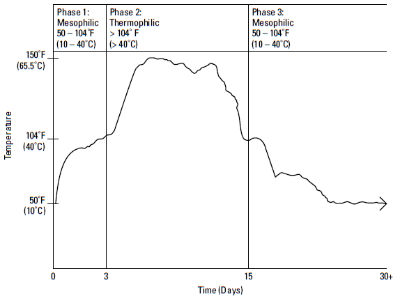
\includegraphics[scale=0.55]{model-T.jpg}
	\caption{Temperature curve for a composting process, \cite{dummies}}
	\label{fig:corba model}
\end{figure}

\subsubsection{Other aspects}
\begin{itemize}
	\item \textbf{Moisture.} Decomposition occurs more rapidly in the thin water films in the surface of the organic particles. Optimal moisture is found to be between 50 and 60\%.
	\item  \textbf{Aeration.} Oxygen is essential for the metabolism and respiration of aerobic organisms and for oxidizing the organic molecules of the waste material. During the process, \ch{O2} is consumed while \ch{CO2} is released. Various methods can be used to maintain the aerobic conditions necessary for the composting process to occur: aeration pipes, air holes, forced air flow or mechanical turning of the pile.
	\item  \textbf{Size of the compost system.} The size of the pile must be small enough to allow aeration through the pile, yet it needs to be of a sufficient size to prevent dissipation of heat.
	\end{itemize}

\section{Development of the model}
\subsection{General approach}
We will base our model on the energy balance of the heat pile. We will consider the pile as an homogeneous system, therefore there will be no spatial dependence for the temperature nor will we consider diffusive processes of the oxygen and other fluids inside the pile. There are two main terms at play: the heat produced by the biochemical process of composting, \( \dot{Q}_c \) and the heat losses of the pile, \( \dot{Q}_l \). We can thus write
\begin{equation} \label{eq:first balance}
	\dot{Q} = \dot{Q}_c + \dot{Q}_l. 
\end{equation}

Given that we are assuming that the pile is homogeneous, we can write the left hand side of \cref{eq:first balance} as \( \dot{Q} = mc\dot{T} \), where \( m \) is the mass of the pile and \( c \) its specific heat capacity. 

As for the losses, given the temperature range we are considering, \SIrange{20}{70}{\celsius}, it seems reasonable to assume that radiation plays no role and that these are mainly due to convection. Since part of the pile will be in contact with the ground, there is conduction taking place. However we will disregard it given that it is a much slower process than convection.  Thus we may write \( \dot{Q}_l = -hA\left(T - T_\text{env}\right) \), where \( h \) is the heat transfer coefficient of air, in \si{W.m^{-1}.K^{-1}}, \( A \) is the exposed surface area of the pile and \( T_\text{env} \) is the outside temperature. We will introduce a sinusoidal time dependence in the ambient temperature to model the given day-night shift between \SI{5}{\celsius} and \SI{20}{\celsius} so 
\begin{align} \label{eq:temp ambient}
	\begin{aligned}
		T_\text{env}(t)  & = \frac{T_\text{max} + T_\text{min}}{2} \\
									 	 & + \frac{T_\text{max} - T_\text{min}}{2} \sin{\left(\frac{2\pi t}{24}\right)},
	\end{aligned}
\end{align}
where \( t \) is the time in hours. 

If the chemical processes involved in composting have an exothermicity of \( Q_b \) then we can write	\( \dot{Q}_c = mQ_b \dot{B} \), where \( B \) is the percentage of mass of the microbial population. The task then is to determine an expression for \( \dot{B} \) that accurately describes the kinetic properties of microbial growth in composting processes.

\subsection{Determining the microbial growth rate}
It seems reasonable to assume that the evolution of the population should be logistic, given that composting entails the depletion of the organic compounds that serve as sustenance to the population. However, the growth should also be tightly coupled to the temperature, so that it reflects the temperature range in which the various populations thrive. The process that limits the growth can be though of as an enzymatic reaction between the two states of the microbes: active, in which they are consuming organic matter and so reproducing, and inactive, in which they are not, as described in \cite{85bio}. \cite{biokinetics} details the kinetics of this kind of processes. Thus the effect of temperature on microbial activity can be evaluated by considering the activation-inactivation reaction,
\begin{equation*}
    \ce{A <=>[\ce{k1}][\ce{k2}] I}. 
\end{equation*}
We have that $\dot{B}=k_1[A]$, since \( [A] \) is the fraction of the microbial population that is reproducing, and $\dot{B}= -k_2[I]$. Additionally, \( [A] + [I] = B \).  By combining these last three equations we have that
\begin{equation} \label{eq:cinetica 1}
	\left(\frac{1}{k_1}-\frac{1}{k_2}\right)\dot{B}=B.
\end{equation}
and 
\begin{equation} \label{eq:cinetica 2}
	k_1[A]+k_2[I]=0.
\end{equation}

If the forward and inverse reactions follow Arrhenius kinetics, we can write $k_i=P_ie^{-E_i/RT}$, where $P_i$ are the empirical pre-exponential factors, $E_i$ the respective activation energies, $R$ the universal gas constant and $T$ the temperature. This, combined with \cref{eq:cinetica 1,eq:cinetica 2} gives the temperature dependance of the specific growth rate \( \mu(T) \), 
\begin{equation} \label{eq:mumax}
    \mu(T)=\frac{P_1e^{-E_1/RT}}{1+\frac{P_2}{P_2}e^{-E_2/RT}}
\end{equation}
using the approximation $k_2\gg k_1$ ACABAR!!!!!

We now have an expression governing the evolution of the bacterial population,
\begin{equation}\label{eq:edo B}
	\dot{B} = \mu(T)B\left(1 - \frac{B}{B_\text{max}}\right),
\end{equation}
which gives us a specific form of the heat generated by the biological process. This form for the biologically generated heat appears in \cite{semenov}. There are additional terms that could be considered. \cite{semenov} uses the heat generated through the microbes' consumption of cellulose. We found that it is, however, much smaller when compared to the term we have obtained.  

Hence, we can write the differential equation that governs \( T \): 
\begin{equation} \label{eq:edo T}
	\begin{aligned}
		mc\dot{T} & = -hA\left(T - T_\text{env}(t)\right) \\
							& + Q_bm\mu(T)B(t)\left(1 - \frac{1}{B_\text{max}}\right). 
	\end{aligned}
\end{equation}
	This is coupled to \cref{eq:edo B}, which governs the growth of the mictrobial population.  

	This equation, however, only accounts for one microbial population. We have mentioned before that composting is a process that takes place in two different stages because there are two different kinds of organisms at play. A way of accounting for this fact in our model is to decouple \( B \) into \( B_1 \), the proportion of mesophilic microorganisms, and \( B_2 \), the proportion of thermophilic microorganisms, each with the correspoding exothermicities and specific growth rates. 

\subsection{Choice of parameters}
\cite{saucedo} gives the preexponential factors, activation energies for the fungus \textit{Aspergillus niger}. This species is mesophilic and proliferates in vegetable waste, specially lettuce, tomato and lemon. This means that we can certainly use this data since we are modeling the composting of domestic vegetable waste. 

No equivalent set of data for thermophilic microbes was readily available. For our model we extrapolated the corresponding parameters for a thermophilic population. Given that the thermophilic phase usually is longer and entails a smaller temperature change than the mesophilic phase, the specific growth rate and exothermicity of thermophiles should be smaller than those of mesophiles. 

In \cite{saucedo}, there is no distinction between mesophiles and thermophiles. It provides values for the initial and maximum concentration for the total microbial population. It seems reasonable to split these values between the mesophilic and thermophilic populations, since we could not find specific data for the ratio of mesophiles to thermophiles. Additionally, these values are given as percentages of the dry matter. Although it is widely known that the moisture content of the composting materials diminishes due to evaporation, we can argue, following \cite{niceassumptions}, that in our case it will remain constant since our pile is not physically isolated from the environment. We assume that the moisture content of vegetable waste is around 50\%. 

\section{Results and analysis}
\begin{figure}[htb]
	\sffamily \footnotesize \centering
	% GNUPLOT: LaTeX picture with Postscript
\begingroup
  \makeatletter
  \providecommand\color[2][]{%
    \GenericError{(gnuplot) \space\space\space\@spaces}{%
      Package color not loaded in conjunction with
      terminal option `colourtext'%
    }{See the gnuplot documentation for explanation.%
    }{Either use 'blacktext' in gnuplot or load the package
      color.sty in LaTeX.}%
    \renewcommand\color[2][]{}%
  }%
  \providecommand\includegraphics[2][]{%
    \GenericError{(gnuplot) \space\space\space\@spaces}{%
      Package graphicx or graphics not loaded%
    }{See the gnuplot documentation for explanation.%
    }{The gnuplot epslatex terminal needs graphicx.sty or graphics.sty.}%
    \renewcommand\includegraphics[2][]{}%
  }%
  \providecommand\rotatebox[2]{#2}%
  \@ifundefined{ifGPcolor}{%
    \newif\ifGPcolor
    \GPcolortrue
  }{}%
  \@ifundefined{ifGPblacktext}{%
    \newif\ifGPblacktext
    \GPblacktextfalse
  }{}%
  % define a \g@addto@macro without @ in the name:
  \let\gplgaddtomacro\g@addto@macro
  % define empty templates for all commands taking text:
  \gdef\gplbacktext{}%
  \gdef\gplfronttext{}%
  \makeatother
  \ifGPblacktext
    % no textcolor at all
    \def\colorrgb#1{}%
    \def\colorgray#1{}%
  \else
    % gray or color?
    \ifGPcolor
      \def\colorrgb#1{\color[rgb]{#1}}%
      \def\colorgray#1{\color[gray]{#1}}%
      \expandafter\def\csname LTw\endcsname{\color{white}}%
      \expandafter\def\csname LTb\endcsname{\color{black}}%
      \expandafter\def\csname LTa\endcsname{\color{black}}%
      \expandafter\def\csname LT0\endcsname{\color[rgb]{1,0,0}}%
      \expandafter\def\csname LT1\endcsname{\color[rgb]{0,1,0}}%
      \expandafter\def\csname LT2\endcsname{\color[rgb]{0,0,1}}%
      \expandafter\def\csname LT3\endcsname{\color[rgb]{1,0,1}}%
      \expandafter\def\csname LT4\endcsname{\color[rgb]{0,1,1}}%
      \expandafter\def\csname LT5\endcsname{\color[rgb]{1,1,0}}%
      \expandafter\def\csname LT6\endcsname{\color[rgb]{0,0,0}}%
      \expandafter\def\csname LT7\endcsname{\color[rgb]{1,0.3,0}}%
      \expandafter\def\csname LT8\endcsname{\color[rgb]{0.5,0.5,0.5}}%
    \else
      % gray
      \def\colorrgb#1{\color{black}}%
      \def\colorgray#1{\color[gray]{#1}}%
      \expandafter\def\csname LTw\endcsname{\color{white}}%
      \expandafter\def\csname LTb\endcsname{\color{black}}%
      \expandafter\def\csname LTa\endcsname{\color{black}}%
      \expandafter\def\csname LT0\endcsname{\color{black}}%
      \expandafter\def\csname LT1\endcsname{\color{black}}%
      \expandafter\def\csname LT2\endcsname{\color{black}}%
      \expandafter\def\csname LT3\endcsname{\color{black}}%
      \expandafter\def\csname LT4\endcsname{\color{black}}%
      \expandafter\def\csname LT5\endcsname{\color{black}}%
      \expandafter\def\csname LT6\endcsname{\color{black}}%
      \expandafter\def\csname LT7\endcsname{\color{black}}%
      \expandafter\def\csname LT8\endcsname{\color{black}}%
    \fi
  \fi
    \setlength{\unitlength}{0.0500bp}%
    \ifx\gptboxheight\undefined%
      \newlength{\gptboxheight}%
      \newlength{\gptboxwidth}%
      \newsavebox{\gptboxtext}%
    \fi%
    \setlength{\fboxrule}{0.5pt}%
    \setlength{\fboxsep}{1pt}%
\begin{picture}(4420.00,3400.00)%
    \gplgaddtomacro\gplbacktext{%
      \csname LTb\endcsname%%
      \put(420,380){\makebox(0,0)[r]{\strut{}\num{10}}}%
      \csname LTb\endcsname%%
      \put(420,702){\makebox(0,0)[r]{\strut{}\num{15}}}%
      \csname LTb\endcsname%%
      \put(420,1024){\makebox(0,0)[r]{\strut{}\num{20}}}%
      \csname LTb\endcsname%%
      \put(420,1347){\makebox(0,0)[r]{\strut{}\num{25}}}%
      \csname LTb\endcsname%%
      \put(420,1669){\makebox(0,0)[r]{\strut{}\num{30}}}%
      \csname LTb\endcsname%%
      \put(420,1991){\makebox(0,0)[r]{\strut{}\num{35}}}%
      \csname LTb\endcsname%%
      \put(420,2313){\makebox(0,0)[r]{\strut{}\num{40}}}%
      \csname LTb\endcsname%%
      \put(420,2636){\makebox(0,0)[r]{\strut{}\num{45}}}%
      \csname LTb\endcsname%%
      \put(420,2958){\makebox(0,0)[r]{\strut{}\num{50}}}%
      \csname LTb\endcsname%%
      \put(420,3280){\makebox(0,0)[r]{\strut{}\num{55}}}%
      \csname LTb\endcsname%%
      \put(487,261){\makebox(0,0){\strut{}\num{0}}}%
      \csname LTb\endcsname%%
      \put(1089,261){\makebox(0,0){\strut{}\num{5}}}%
      \csname LTb\endcsname%%
      \put(1691,261){\makebox(0,0){\strut{}\num{10}}}%
      \csname LTb\endcsname%%
      \put(2292,261){\makebox(0,0){\strut{}\num{15}}}%
      \csname LTb\endcsname%%
      \put(2894,261){\makebox(0,0){\strut{}\num{20}}}%
      \csname LTb\endcsname%%
      \put(3496,261){\makebox(0,0){\strut{}\num{25}}}%
      \csname LTb\endcsname%%
      \put(4098,261){\makebox(0,0){\strut{}\num{30}}}%
    }%
    \gplgaddtomacro\gplfronttext{%
      \csname LTb\endcsname%%
      \put(100,1830){\rotatebox{-270}{\makebox(0,0){\strut{}$\mathsfit T \ (\si{\celsius})$}}}%
      \csname LTb\endcsname%%
      \put(2352,83){\makebox(0,0){\strut{}$\mathsfit t \ (\si{days})$}}%
    }%
    \gplbacktext
    \put(0,0){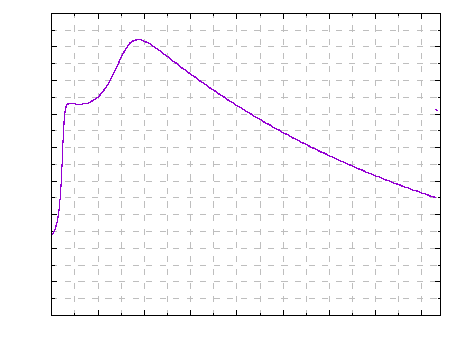
\includegraphics{2-temperatura}}%
    \gplfronttext
  \end{picture}%
\endgroup

	\caption{Temperature evolution of the compost pile modeled with mesophilic and thermophilic populations}
	\label{fig:temp-mesos-termos}
\end{figure}

\subsection{Analysis of a generic composting process}
Considering a compost pile of a surface area of \SI{7}{m^2} with \SI{30}{kg} inside, we obtain the temperature profile in \cref{fig:temp-mesos-termos}. One can clearly observe the three different phases of the composting process. During the first 48 hours the temperature rises rapidly due to the burst in activity of the mesophilic population. This is also clear in \cref{fig:potencies}. We can see that the mesophilic population outputs the highest power during the first 24 hours but quickly decays as the mesophilic population reaches its saturation value and becomes stagnant.

After this, the thermophilic activity rises. Given that we modeled the thermophilic process to be much slower and less exothermic than the mesophilic one, the maximum output power is not nearly as high, nor is the decay as stark. This explains the slight dip in the temperature we observe after the mesophilic activity ceases: the power output by the thermophilic process in its initial stage is too low to counter the heat lost due to convection, therefore the temperature dips. After this, however, the temperature rises steadily to just under \SI{50}{\celsius}. We see that thermophilic activity diminishes after 12 days, when the population reaches its saturation value (\cref{fig:poblacions}). 

\begin{figure}[htb]
	\sffamily \footnotesize \centering
	% GNUPLOT: LaTeX picture with Postscript
\begingroup
\newcommand{\etiqueta}[1]{\setlength{\fboxsep}{0.75pt}\colorbox{white}{#1}}
  \makeatletter
  \providecommand\color[2][]{%
    \GenericError{(gnuplot) \space\space\space\@spaces}{%
      Package color not loaded in conjunction with
      terminal option `colourtext'%
    }{See the gnuplot documentation for explanation.%
    }{Either use 'blacktext' in gnuplot or load the package
      color.sty in LaTeX.}%
    \renewcommand\color[2][]{}%
  }%
  \providecommand\includegraphics[2][]{%
    \GenericError{(gnuplot) \space\space\space\@spaces}{%
      Package graphicx or graphics not loaded%
    }{See the gnuplot documentation for explanation.%
    }{The gnuplot epslatex terminal needs graphicx.sty or graphics.sty.}%
    \renewcommand\includegraphics[2][]{}%
  }%
  \providecommand\rotatebox[2]{#2}%
  \@ifundefined{ifGPcolor}{%
    \newif\ifGPcolor
    \GPcolortrue
  }{}%
  \@ifundefined{ifGPblacktext}{%
    \newif\ifGPblacktext
    \GPblacktextfalse
  }{}%
  % define a \g@addto@macro without @ in the name:
  \let\gplgaddtomacro\g@addto@macro
  % define empty templates for all commands taking text:
  \gdef\gplbacktext{}%
  \gdef\gplfronttext{}%
  \makeatother
  \ifGPblacktext
    % no textcolor at all
    \def\colorrgb#1{}%
    \def\colorgray#1{}%
  \else
    % gray or color?
    \ifGPcolor
      \def\colorrgb#1{\color[rgb]{#1}}%
      \def\colorgray#1{\color[gray]{#1}}%
      \expandafter\def\csname LTw\endcsname{\color{white}}%
      \expandafter\def\csname LTb\endcsname{\color{black}}%
      \expandafter\def\csname LTa\endcsname{\color{black}}%
      \expandafter\def\csname LT0\endcsname{\color[rgb]{1,0,0}}%
      \expandafter\def\csname LT1\endcsname{\color[rgb]{0,1,0}}%
      \expandafter\def\csname LT2\endcsname{\color[rgb]{0,0,1}}%
      \expandafter\def\csname LT3\endcsname{\color[rgb]{1,0,1}}%
      \expandafter\def\csname LT4\endcsname{\color[rgb]{0,1,1}}%
      \expandafter\def\csname LT5\endcsname{\color[rgb]{1,1,0}}%
      \expandafter\def\csname LT6\endcsname{\color[rgb]{0,0,0}}%
      \expandafter\def\csname LT7\endcsname{\color[rgb]{1,0.3,0}}%
      \expandafter\def\csname LT8\endcsname{\color[rgb]{0.5,0.5,0.5}}%
    \else
      % gray
      \def\colorrgb#1{\color{black}}%
      \def\colorgray#1{\color[gray]{#1}}%
      \expandafter\def\csname LTw\endcsname{\color{white}}%
      \expandafter\def\csname LTb\endcsname{\color{black}}%
      \expandafter\def\csname LTa\endcsname{\color{black}}%
      \expandafter\def\csname LT0\endcsname{\color{black}}%
      \expandafter\def\csname LT1\endcsname{\color{black}}%
      \expandafter\def\csname LT2\endcsname{\color{black}}%
      \expandafter\def\csname LT3\endcsname{\color{black}}%
      \expandafter\def\csname LT4\endcsname{\color{black}}%
      \expandafter\def\csname LT5\endcsname{\color{black}}%
      \expandafter\def\csname LT6\endcsname{\color{black}}%
      \expandafter\def\csname LT7\endcsname{\color{black}}%
      \expandafter\def\csname LT8\endcsname{\color{black}}%
    \fi
  \fi
    \setlength{\unitlength}{0.0500bp}%
    \ifx\gptboxheight\undefined%
      \newlength{\gptboxheight}%
      \newlength{\gptboxwidth}%
      \newsavebox{\gptboxtext}%
    \fi%
    \setlength{\fboxrule}{0.5pt}%
    \setlength{\fboxsep}{1pt}%
\begin{picture}(4420.00,3400.00)%
    \gplgaddtomacro\gplbacktext{%
      \csname LTb\endcsname%%
      \put(487,380){\makebox(0,0)[r]{\strut{}\num{0}}}%
      \csname LTb\endcsname%%
      \put(487,743){\makebox(0,0)[r]{\strut{}\num{20}}}%
      \csname LTb\endcsname%%
      \put(487,1105){\makebox(0,0)[r]{\strut{}\num{40}}}%
      \csname LTb\endcsname%%
      \put(487,1468){\makebox(0,0)[r]{\strut{}\num{60}}}%
      \csname LTb\endcsname%%
      \put(487,1830){\makebox(0,0)[r]{\strut{}\num{80}}}%
      \csname LTb\endcsname%%
      \put(487,2193){\makebox(0,0)[r]{\strut{}\num{100}}}%
      \csname LTb\endcsname%%
      \put(487,2555){\makebox(0,0)[r]{\strut{}\num{120}}}%
      \csname LTb\endcsname%%
      \put(487,2918){\makebox(0,0)[r]{\strut{}\num{140}}}%
      \csname LTb\endcsname%%
      \put(487,3280){\makebox(0,0)[r]{\strut{}\num{160}}}%
      \csname LTb\endcsname%%
      \put(554,261){\makebox(0,0){\strut{}\num{0}}}%
      \csname LTb\endcsname%%
      \put(1077,261){\makebox(0,0){\strut{}\num{2}}}%
      \csname LTb\endcsname%%
      \put(1601,261){\makebox(0,0){\strut{}\num{4}}}%
      \csname LTb\endcsname%%
      \put(2124,261){\makebox(0,0){\strut{}\num{6}}}%
      \csname LTb\endcsname%%
      \put(2648,261){\makebox(0,0){\strut{}\num{8}}}%
      \csname LTb\endcsname%%
      \put(3171,261){\makebox(0,0){\strut{}\num{10}}}%
      \csname LTb\endcsname%%
      \put(3695,261){\makebox(0,0){\strut{}\num{12}}}%
      \csname LTb\endcsname%%
      \put(4218,261){\makebox(0,0){\strut{}\num{14}}}%
    }%
    \gplgaddtomacro\gplfronttext{%
      \csname LTb\endcsname%%
      \put(100,1830){\rotatebox{-270}{\makebox(0,0){\strut{}$\mathsfit P \ (\si{kW})$}}}%
      \csname LTb\endcsname%%
      \put(2386,83){\makebox(0,0){\strut{}$\mathsfit t \ (\si{days})$}}%
      \csname LTb\endcsname%%
      \put(1077,1830){\rotatebox{-87}{\makebox(0,0){\strut{}\etiqueta{\footnotesize Mesophiles}}}}%
      \csname LTb\endcsname%%
      \put(1863,688){\rotatebox{10}{\makebox(0,0){\strut{}\etiqueta{\footnotesize Thermophiles}}}}%
    }%
    \gplbacktext
    \put(0,0){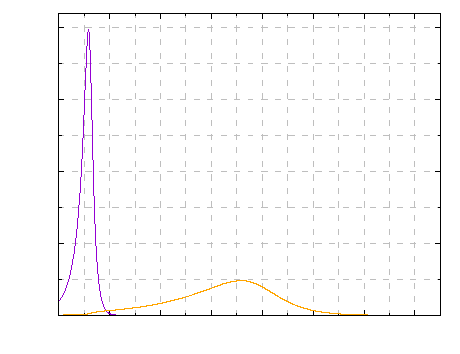
\includegraphics{2-potencies}}%
    \gplfronttext
  \end{picture}%
\endgroup

	\caption{Power output of the mesophilic and thermophilic reactions}
	\label{fig:potencies}
\end{figure}

After this point, the pile is subject solely to convective losses, and its temperature slowly decays to the ambient temperature. It must be noted that the temperature does suffer small fluctuations ---within \SI{1}{\celsius}--- due to the oscillation of the ambient temperature. However the oscillations of the outside temperature are too fast ---they have a period of 1 day--- to have a significant effect on the temperature of the pile.  

\begin{figure}[htb]
	\sffamily \footnotesize \centering
	% GNUPLOT: LaTeX picture with Postscript
\begingroup
\newcommand{\etiqueta}[1]{\setlength{\fboxsep}{0.75pt}\colorbox{white}{#1}}
  \makeatletter
  \providecommand\color[2][]{%
    \GenericError{(gnuplot) \space\space\space\@spaces}{%
      Package color not loaded in conjunction with
      terminal option `colourtext'%
    }{See the gnuplot documentation for explanation.%
    }{Either use 'blacktext' in gnuplot or load the package
      color.sty in LaTeX.}%
    \renewcommand\color[2][]{}%
  }%
  \providecommand\includegraphics[2][]{%
    \GenericError{(gnuplot) \space\space\space\@spaces}{%
      Package graphicx or graphics not loaded%
    }{See the gnuplot documentation for explanation.%
    }{The gnuplot epslatex terminal needs graphicx.sty or graphics.sty.}%
    \renewcommand\includegraphics[2][]{}%
  }%
  \providecommand\rotatebox[2]{#2}%
  \@ifundefined{ifGPcolor}{%
    \newif\ifGPcolor
    \GPcolortrue
  }{}%
  \@ifundefined{ifGPblacktext}{%
    \newif\ifGPblacktext
    \GPblacktextfalse
  }{}%
  % define a \g@addto@macro without @ in the name:
  \let\gplgaddtomacro\g@addto@macro
  % define empty templates for all commands taking text:
  \gdef\gplbacktext{}%
  \gdef\gplfronttext{}%
  \makeatother
  \ifGPblacktext
    % no textcolor at all
    \def\colorrgb#1{}%
    \def\colorgray#1{}%
  \else
    % gray or color?
    \ifGPcolor
      \def\colorrgb#1{\color[rgb]{#1}}%
      \def\colorgray#1{\color[gray]{#1}}%
      \expandafter\def\csname LTw\endcsname{\color{white}}%
      \expandafter\def\csname LTb\endcsname{\color{black}}%
      \expandafter\def\csname LTa\endcsname{\color{black}}%
      \expandafter\def\csname LT0\endcsname{\color[rgb]{1,0,0}}%
      \expandafter\def\csname LT1\endcsname{\color[rgb]{0,1,0}}%
      \expandafter\def\csname LT2\endcsname{\color[rgb]{0,0,1}}%
      \expandafter\def\csname LT3\endcsname{\color[rgb]{1,0,1}}%
      \expandafter\def\csname LT4\endcsname{\color[rgb]{0,1,1}}%
      \expandafter\def\csname LT5\endcsname{\color[rgb]{1,1,0}}%
      \expandafter\def\csname LT6\endcsname{\color[rgb]{0,0,0}}%
      \expandafter\def\csname LT7\endcsname{\color[rgb]{1,0.3,0}}%
      \expandafter\def\csname LT8\endcsname{\color[rgb]{0.5,0.5,0.5}}%
    \else
      % gray
      \def\colorrgb#1{\color{black}}%
      \def\colorgray#1{\color[gray]{#1}}%
      \expandafter\def\csname LTw\endcsname{\color{white}}%
      \expandafter\def\csname LTb\endcsname{\color{black}}%
      \expandafter\def\csname LTa\endcsname{\color{black}}%
      \expandafter\def\csname LT0\endcsname{\color{black}}%
      \expandafter\def\csname LT1\endcsname{\color{black}}%
      \expandafter\def\csname LT2\endcsname{\color{black}}%
      \expandafter\def\csname LT3\endcsname{\color{black}}%
      \expandafter\def\csname LT4\endcsname{\color{black}}%
      \expandafter\def\csname LT5\endcsname{\color{black}}%
      \expandafter\def\csname LT6\endcsname{\color{black}}%
      \expandafter\def\csname LT7\endcsname{\color{black}}%
      \expandafter\def\csname LT8\endcsname{\color{black}}%
    \fi
  \fi
    \setlength{\unitlength}{0.0500bp}%
    \ifx\gptboxheight\undefined%
      \newlength{\gptboxheight}%
      \newlength{\gptboxwidth}%
      \newsavebox{\gptboxtext}%
    \fi%
    \setlength{\fboxrule}{0.5pt}%
    \setlength{\fboxsep}{1pt}%
\begin{picture}(4420.00,3400.00)%
    \gplgaddtomacro\gplbacktext{%
      \csname LTb\endcsname%%
      \put(435,380){\makebox(0,0)[r]{\strut{}\num{0}}}%
      \csname LTb\endcsname%%
      \put(435,743){\makebox(0,0)[r]{\strut{}\num{0.01}}}%
      \csname LTb\endcsname%%
      \put(435,1105){\makebox(0,0)[r]{\strut{}\num{0.02}}}%
      \csname LTb\endcsname%%
      \put(435,1468){\makebox(0,0)[r]{\strut{}\num{0.03}}}%
      \csname LTb\endcsname%%
      \put(435,1830){\makebox(0,0)[r]{\strut{}\num{0.04}}}%
      \csname LTb\endcsname%%
      \put(435,2193){\makebox(0,0)[r]{\strut{}\num{0.05}}}%
      \csname LTb\endcsname%%
      \put(435,2555){\makebox(0,0)[r]{\strut{}\num{0.06}}}%
      \csname LTb\endcsname%%
      \put(435,2918){\makebox(0,0)[r]{\strut{}\num{0.07}}}%
      \csname LTb\endcsname%%
      \put(435,3280){\makebox(0,0)[r]{\strut{}\num{0.08}}}%
      \csname LTb\endcsname%%
      \put(502,261){\makebox(0,0){\strut{}\num{0}}}%
      \csname LTb\endcsname%%
      \put(997,261){\makebox(0,0){\strut{}\num{2}}}%
      \csname LTb\endcsname%%
      \put(1493,261){\makebox(0,0){\strut{}\num{4}}}%
      \csname LTb\endcsname%%
      \put(1988,261){\makebox(0,0){\strut{}\num{6}}}%
      \csname LTb\endcsname%%
      \put(2484,261){\makebox(0,0){\strut{}\num{8}}}%
      \csname LTb\endcsname%%
      \put(2979,261){\makebox(0,0){\strut{}\num{10}}}%
      \csname LTb\endcsname%%
      \put(3475,261){\makebox(0,0){\strut{}\num{12}}}%
      \csname LTb\endcsname%%
      \put(3970,261){\makebox(0,0){\strut{}\num{14}}}%
    }%
    \gplgaddtomacro\gplfronttext{%
      \csname LTb\endcsname%%
      \put(2360,83){\makebox(0,0){\strut{}$\mathsfit t \ (\si{days})$}}%
      \csname LTb\endcsname%%
      \put(997,1830){\rotatebox{85}{\makebox(0,0){\strut{}\etiqueta{\footnotesize Mesophiles}}}}%
      \csname LTb\endcsname%%
      \put(2484,1830){\rotatebox{65}{\makebox(0,0){\strut{}\etiqueta{\footnotesize Thermophiles}}}}%
    }%
    \gplbacktext
    \put(0,0){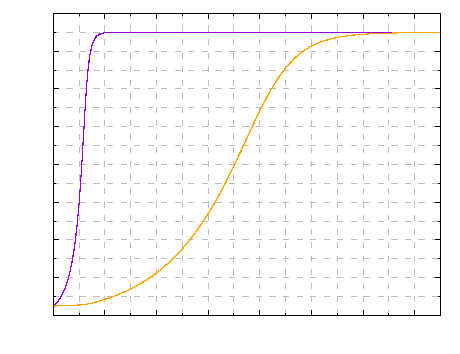
\includegraphics{2-bacteris}}%
    \gplfronttext
  \end{picture}%
\endgroup

	\caption{Evolution of the relative mass of the populations of mesophilic and thermophilic organisms}
	\label{fig:poblacions}
\end{figure}

\subsection{Analysis of the dimensions of the pile}
Given that we are considering composting on the domestic scale, the range of sizes of the pile is rather limited. If we assume a cubic pile, then a surface area of \SI{10}{m^2}	entails a side length of about \SI{1.3}{m}, which would be on the edge of practicality for the domestic scale. We will therefore only consider surface areas within this range. 

\begin{figure}[htb]
	\sffamily \footnotesize \centering
	% GNUPLOT: LaTeX picture with Postscript
\begingroup
\newcommand{\etiqueta}[1]{\setlength{\fboxsep}{0.75pt}\colorbox{white}{#1}}
  \makeatletter
  \providecommand\color[2][]{%
    \GenericError{(gnuplot) \space\space\space\@spaces}{%
      Package color not loaded in conjunction with
      terminal option `colourtext'%
    }{See the gnuplot documentation for explanation.%
    }{Either use 'blacktext' in gnuplot or load the package
      color.sty in LaTeX.}%
    \renewcommand\color[2][]{}%
  }%
  \providecommand\includegraphics[2][]{%
    \GenericError{(gnuplot) \space\space\space\@spaces}{%
      Package graphicx or graphics not loaded%
    }{See the gnuplot documentation for explanation.%
    }{The gnuplot epslatex terminal needs graphicx.sty or graphics.sty.}%
    \renewcommand\includegraphics[2][]{}%
  }%
  \providecommand\rotatebox[2]{#2}%
  \@ifundefined{ifGPcolor}{%
    \newif\ifGPcolor
    \GPcolortrue
  }{}%
  \@ifundefined{ifGPblacktext}{%
    \newif\ifGPblacktext
    \GPblacktextfalse
  }{}%
  % define a \g@addto@macro without @ in the name:
  \let\gplgaddtomacro\g@addto@macro
  % define empty templates for all commands taking text:
  \gdef\gplbacktext{}%
  \gdef\gplfronttext{}%
  \makeatother
  \ifGPblacktext
    % no textcolor at all
    \def\colorrgb#1{}%
    \def\colorgray#1{}%
  \else
    % gray or color?
    \ifGPcolor
      \def\colorrgb#1{\color[rgb]{#1}}%
      \def\colorgray#1{\color[gray]{#1}}%
      \expandafter\def\csname LTw\endcsname{\color{white}}%
      \expandafter\def\csname LTb\endcsname{\color{black}}%
      \expandafter\def\csname LTa\endcsname{\color{black}}%
      \expandafter\def\csname LT0\endcsname{\color[rgb]{1,0,0}}%
      \expandafter\def\csname LT1\endcsname{\color[rgb]{0,1,0}}%
      \expandafter\def\csname LT2\endcsname{\color[rgb]{0,0,1}}%
      \expandafter\def\csname LT3\endcsname{\color[rgb]{1,0,1}}%
      \expandafter\def\csname LT4\endcsname{\color[rgb]{0,1,1}}%
      \expandafter\def\csname LT5\endcsname{\color[rgb]{1,1,0}}%
      \expandafter\def\csname LT6\endcsname{\color[rgb]{0,0,0}}%
      \expandafter\def\csname LT7\endcsname{\color[rgb]{1,0.3,0}}%
      \expandafter\def\csname LT8\endcsname{\color[rgb]{0.5,0.5,0.5}}%
    \else
      % gray
      \def\colorrgb#1{\color{black}}%
      \def\colorgray#1{\color[gray]{#1}}%
      \expandafter\def\csname LTw\endcsname{\color{white}}%
      \expandafter\def\csname LTb\endcsname{\color{black}}%
      \expandafter\def\csname LTa\endcsname{\color{black}}%
      \expandafter\def\csname LT0\endcsname{\color{black}}%
      \expandafter\def\csname LT1\endcsname{\color{black}}%
      \expandafter\def\csname LT2\endcsname{\color{black}}%
      \expandafter\def\csname LT3\endcsname{\color{black}}%
      \expandafter\def\csname LT4\endcsname{\color{black}}%
      \expandafter\def\csname LT5\endcsname{\color{black}}%
      \expandafter\def\csname LT6\endcsname{\color{black}}%
      \expandafter\def\csname LT7\endcsname{\color{black}}%
      \expandafter\def\csname LT8\endcsname{\color{black}}%
    \fi
  \fi
    \setlength{\unitlength}{0.0500bp}%
    \ifx\gptboxheight\undefined%
      \newlength{\gptboxheight}%
      \newlength{\gptboxwidth}%
      \newsavebox{\gptboxtext}%
    \fi%
    \setlength{\fboxrule}{0.5pt}%
    \setlength{\fboxsep}{1pt}%
\begin{picture}(4420.00,3400.00)%
    \gplgaddtomacro\gplbacktext{%
      \csname LTb\endcsname%%
      \put(420,380){\makebox(0,0)[r]{\strut{}\num{10}}}%
      \csname LTb\endcsname%%
      \put(420,907){\makebox(0,0)[r]{\strut{}\num{20}}}%
      \csname LTb\endcsname%%
      \put(420,1435){\makebox(0,0)[r]{\strut{}\num{30}}}%
      \csname LTb\endcsname%%
      \put(420,1962){\makebox(0,0)[r]{\strut{}\num{40}}}%
      \csname LTb\endcsname%%
      \put(420,2489){\makebox(0,0)[r]{\strut{}\num{50}}}%
      \csname LTb\endcsname%%
      \put(420,3016){\makebox(0,0)[r]{\strut{}\num{60}}}%
      \csname LTb\endcsname%%
      \put(487,261){\makebox(0,0){\strut{}\num{0}}}%
      \csname LTb\endcsname%%
      \put(1089,261){\makebox(0,0){\strut{}\num{5}}}%
      \csname LTb\endcsname%%
      \put(1691,261){\makebox(0,0){\strut{}\num{10}}}%
      \csname LTb\endcsname%%
      \put(2292,261){\makebox(0,0){\strut{}\num{15}}}%
      \csname LTb\endcsname%%
      \put(2894,261){\makebox(0,0){\strut{}\num{20}}}%
      \csname LTb\endcsname%%
      \put(3496,261){\makebox(0,0){\strut{}\num{25}}}%
      \csname LTb\endcsname%%
      \put(4098,261){\makebox(0,0){\strut{}\num{30}}}%
    }%
    \gplgaddtomacro\gplfronttext{%
      \csname LTb\endcsname%%
      \put(100,1830){\rotatebox{-270}{\makebox(0,0){\strut{}$\mathsfit T \ (\si{\celsius})$}}}%
      \csname LTb\endcsname%%
      \put(2352,83){\makebox(0,0){\strut{}$\mathsfit t \ (\si{days})$}}%
      \csname LTb\endcsname%%
      \put(3737,3069){\rotatebox{-5}{\makebox(0,0){\strut{}\etiqueta{\footnotesize $\mathsfit{A} = \SI{1}{m^2}$}}}}%
      \csname LTb\endcsname%%
      \put(2894,1487){\rotatebox{-25}{\makebox(0,0){\strut{}\etiqueta{\footnotesize $\mathsfit{A} = \SI{10}{m^2}$}}}}%
    }%
    \gplbacktext
    \put(0,0){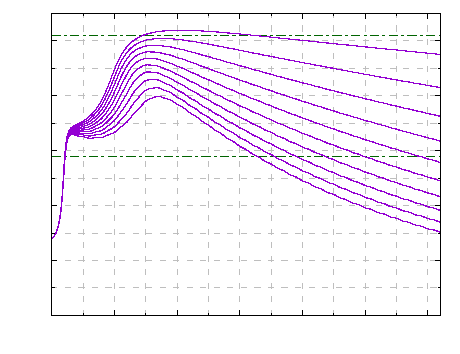
\includegraphics{2-temperatura-A}}%
    \gplfronttext
  \end{picture}%
\endgroup

	\caption{Temperature evolution of the compost pile for various values of surface area}
	\label{fig:temp-arees}
\end{figure}

If we assume the density of vegetable waste to be on the order of \SI{500}{kg.m^{-3}}, for a given value of surface area, we can compute the mass of the pile as \( m = \rho(A/5)^{\frac{3}{2}} \), since only five out of the six faces would suffer heat loss due to convection, the sixth one being in contact with the ground. We see that the temperature evolution during the thermophilic stage is essentially independent of the area, but not the thermophilic stage. The maximum temperature ranges between \SI{50}{\celsius} and \SI{57}{\celsius}, with the higher temperatures being attained for the smaller surface areas which are less subject to convective losses.   

\begin{figure}[htb]
	\sffamily \footnotesize \centering
	% GNUPLOT: LaTeX picture with Postscript
\begingroup
\newcommand{\etiqueta}[1]{\setlength{\fboxsep}{0.75pt}\colorbox{white}{#1}}
  \makeatletter
  \providecommand\color[2][]{%
    \GenericError{(gnuplot) \space\space\space\@spaces}{%
      Package color not loaded in conjunction with
      terminal option `colourtext'%
    }{See the gnuplot documentation for explanation.%
    }{Either use 'blacktext' in gnuplot or load the package
      color.sty in LaTeX.}%
    \renewcommand\color[2][]{}%
  }%
  \providecommand\includegraphics[2][]{%
    \GenericError{(gnuplot) \space\space\space\@spaces}{%
      Package graphicx or graphics not loaded%
    }{See the gnuplot documentation for explanation.%
    }{The gnuplot epslatex terminal needs graphicx.sty or graphics.sty.}%
    \renewcommand\includegraphics[2][]{}%
  }%
  \providecommand\rotatebox[2]{#2}%
  \@ifundefined{ifGPcolor}{%
    \newif\ifGPcolor
    \GPcolortrue
  }{}%
  \@ifundefined{ifGPblacktext}{%
    \newif\ifGPblacktext
    \GPblacktextfalse
  }{}%
  % define a \g@addto@macro without @ in the name:
  \let\gplgaddtomacro\g@addto@macro
  % define empty templates for all commands taking text:
  \gdef\gplbacktext{}%
  \gdef\gplfronttext{}%
  \makeatother
  \ifGPblacktext
    % no textcolor at all
    \def\colorrgb#1{}%
    \def\colorgray#1{}%
  \else
    % gray or color?
    \ifGPcolor
      \def\colorrgb#1{\color[rgb]{#1}}%
      \def\colorgray#1{\color[gray]{#1}}%
      \expandafter\def\csname LTw\endcsname{\color{white}}%
      \expandafter\def\csname LTb\endcsname{\color{black}}%
      \expandafter\def\csname LTa\endcsname{\color{black}}%
      \expandafter\def\csname LT0\endcsname{\color[rgb]{1,0,0}}%
      \expandafter\def\csname LT1\endcsname{\color[rgb]{0,1,0}}%
      \expandafter\def\csname LT2\endcsname{\color[rgb]{0,0,1}}%
      \expandafter\def\csname LT3\endcsname{\color[rgb]{1,0,1}}%
      \expandafter\def\csname LT4\endcsname{\color[rgb]{0,1,1}}%
      \expandafter\def\csname LT5\endcsname{\color[rgb]{1,1,0}}%
      \expandafter\def\csname LT6\endcsname{\color[rgb]{0,0,0}}%
      \expandafter\def\csname LT7\endcsname{\color[rgb]{1,0.3,0}}%
      \expandafter\def\csname LT8\endcsname{\color[rgb]{0.5,0.5,0.5}}%
    \else
      % gray
      \def\colorrgb#1{\color{black}}%
      \def\colorgray#1{\color[gray]{#1}}%
      \expandafter\def\csname LTw\endcsname{\color{white}}%
      \expandafter\def\csname LTb\endcsname{\color{black}}%
      \expandafter\def\csname LTa\endcsname{\color{black}}%
      \expandafter\def\csname LT0\endcsname{\color{black}}%
      \expandafter\def\csname LT1\endcsname{\color{black}}%
      \expandafter\def\csname LT2\endcsname{\color{black}}%
      \expandafter\def\csname LT3\endcsname{\color{black}}%
      \expandafter\def\csname LT4\endcsname{\color{black}}%
      \expandafter\def\csname LT5\endcsname{\color{black}}%
      \expandafter\def\csname LT6\endcsname{\color{black}}%
      \expandafter\def\csname LT7\endcsname{\color{black}}%
      \expandafter\def\csname LT8\endcsname{\color{black}}%
    \fi
  \fi
    \setlength{\unitlength}{0.0500bp}%
    \ifx\gptboxheight\undefined%
      \newlength{\gptboxheight}%
      \newlength{\gptboxwidth}%
      \newsavebox{\gptboxtext}%
    \fi%
    \setlength{\fboxrule}{0.5pt}%
    \setlength{\fboxsep}{1pt}%
\begin{picture}(4420.00,3400.00)%
    \gplgaddtomacro\gplbacktext{%
      \csname LTb\endcsname%%
      \put(420,380){\makebox(0,0)[r]{\strut{}\num{10}}}%
      \csname LTb\endcsname%%
      \put(420,907){\makebox(0,0)[r]{\strut{}\num{20}}}%
      \csname LTb\endcsname%%
      \put(420,1435){\makebox(0,0)[r]{\strut{}\num{30}}}%
      \csname LTb\endcsname%%
      \put(420,1962){\makebox(0,0)[r]{\strut{}\num{40}}}%
      \csname LTb\endcsname%%
      \put(420,2489){\makebox(0,0)[r]{\strut{}\num{50}}}%
      \csname LTb\endcsname%%
      \put(420,3016){\makebox(0,0)[r]{\strut{}\num{60}}}%
      \csname LTb\endcsname%%
      \put(487,261){\makebox(0,0){\strut{}\num{0}}}%
      \csname LTb\endcsname%%
      \put(1089,261){\makebox(0,0){\strut{}\num{5}}}%
      \csname LTb\endcsname%%
      \put(1691,261){\makebox(0,0){\strut{}\num{10}}}%
      \csname LTb\endcsname%%
      \put(2292,261){\makebox(0,0){\strut{}\num{15}}}%
      \csname LTb\endcsname%%
      \put(2894,261){\makebox(0,0){\strut{}\num{20}}}%
      \csname LTb\endcsname%%
      \put(3496,261){\makebox(0,0){\strut{}\num{25}}}%
      \csname LTb\endcsname%%
      \put(4098,261){\makebox(0,0){\strut{}\num{30}}}%
    }%
    \gplgaddtomacro\gplfronttext{%
      \csname LTb\endcsname%%
      \put(100,1830){\rotatebox{-270}{\makebox(0,0){\strut{}$\mathsfit T \ (\si{\celsius})$}}}%
      \csname LTb\endcsname%%
      \put(2352,83){\makebox(0,0){\strut{}$\mathsfit t \ (\si{days})$}}%
      \colorrgb{0.58,0.00,0.83}%%
      \put(3496,2858){\rotatebox{-6}{\makebox(0,0){\strut{}\etiqueta{\footnotesize $\mathsfit{A} = \SI{1}{m^2}$}}}}%
      \colorrgb{0.58,0.00,0.83}%%
      \put(2894,2489){\rotatebox{-13}{\makebox(0,0){\strut{}\etiqueta{\footnotesize $\mathsfit{A} = \SI{10}{m^2}$}}}}%
    }%
    \gplbacktext
    \put(0,0){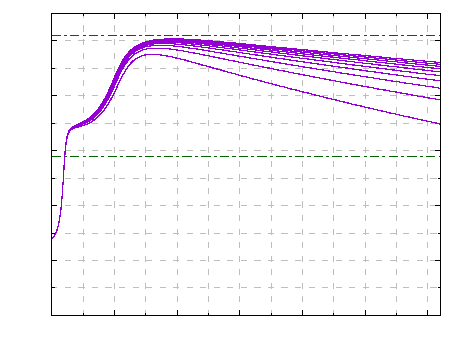
\includegraphics{3-temperatura-A}}%
    \gplfronttext
  \end{picture}%
\endgroup

	\caption{Temperature evolution of the compost pile for various values of surface area}
	\label{fig:temp-semiesferes}
\end{figure}

To obtain \cref{fig:temp-semiesferes} we performed the same calculations considering a semispherical pile instead. The relationship between the mass and the surface area now becomes \( m = \rho\frac{4\pi}{3}(\frac{A}{2\pi})^{\frac{3}{2}} \).

\clearpage
\appendix

\section{References and Further Reading}
\begin{btSect}{fonts}
	\bibliographystyle{ieeetr}
	\subsection*{References}	
	\btPrintCited
\end{btSect}

\begin{btSect}{fonts}
	\bibliographystyle{ieeetr}
	\subsection*{Further Reading}	
	\btPrintNotCited
\end{btSect}

\end{document}
